\chapter{\texorpdfstring{Measuring the CP structure of the Higgs-tau Yukawa coupling in $\PGt_h \PGt_h$ decays}{Measurement of the CP structure of the Higgs-tau Yukawa coupling in tauh tauh decays}}
\chaptermark{\texorpdfstring{Measurement of Higgs CP structure in $H \to \PGt_h \PGt_h$ decays}{Measurement of Higgs CP structure in H to tauh tauh decays}}
\thispagestyle{plain}  % First page has default style
\pagestyle{chapterpages}
\label{Section:Chapter_CP}
\minitoc

\section{Introduction}

As outlined in Section~\ref{Section:Chapter2_CP_Yukawa_Structure}, the CP structure of the Higgs-tau Yukawa coupling can be probed through spin correlations in $H \to \tau\tau$ decays. These correlations are captured in the acoplanarity angle $\phi_{CP}$ between the $\tau^+$ and $\tau^-$ decay planes, which serves as the primary CP-sensitive observable.

In the \ac{SM}, this measurement is expressed in terms of the effective CP mixing angle $\alpha_{\tau\tau}$, predicted to be essentially zero for a purely CP-even interaction. A significant deviation of $\alpha_{\tau\tau}$ from zero would be direct evidence for CP violation in the Higgs–fermion sector, with important implications for physics beyond the \ac{SM}. Minimal supersymmetric models predict only negligible CP-violating effects in Yukawa couplings, whereas extended Higgs sectors such as the next-to-minimal supersymmetric model can accommodate values up to ${\sim}27^\circ$~\cite{King:2015oxa}.

The most precise determination to date was performed by the \ac{CMS} Collaboration using the full Run 2 dataset of $137~\mathrm{fb}^{-1}$ at $\sqrt{s} = 13~\mathrm{TeV}$~\cite{HiggsCP_CMS_2021}. That analysis combined multiple $\tau$ decay channels, including leptonic modes ($\tau_e^\pm,\ \tau_\mu^\pm$) and the dominant hadronic modes ($\pi^\pm$, $\rho^\pm \to \pi^\pm \pi^0$, $a_1^\pm \to \pi^\pm \pi^0 \pi^0$, $a_1^\pm \to \pi^\pm \pi^\mp \pi^\pm$). The result, $\alpha_{\tau\tau} = -1 \pm 19^\circ$ (expected $0 \pm 21^\circ$) at the 68.3\% CL, disfavouring the pure CP-odd scenario at $3.0\sigma$, was dominated by statistical uncertainty. Feasibility studies indicate that a precision of ${\sim}5$-$10^\circ$ could be achieved with $3\unit{ab}^{-1}$ of data~\cite{Harnik:2013aja,Berge:2014sra}.

This chapter presents a complementary measurement targeting only the $\PGt_h \PGt_h$ final state. The dataset corresponds to the partial Run 3 data-taking period and is substantially smaller in integrated luminosity than in Run 2, leading to reduced statistical reach. Despite the smaller dataset, this analysis aims to approach the precision of the Run 2 results by targeting improvements in key components such as:

\begin{enumerate}[label=(\roman*)]
    \item Tau identification
    \item Triggering
    \item Tau DM classification
    \item Event Categorisation
    \item Reconstruction of the sensitive observable
\end{enumerate}

These developments are aimed at paving the way to a competitive measurement well before the \ac{HL}-\ac{LHC} era, and will be discussed in more detail throughout this chapter, along with an improved analysis strategy.

\section{Collision data}

This analysis uses proton–proton collision data recorded by the \ac{CMS} detector during the initial part of the Run 3 period (2022–2023). The collisions were produced at a centre-of-mass energy of $\sqrt{s} = 13.6\TeV$, and the dataset corresponds to an integrated luminosity of about $61.9\unit{fb}^{-1}$.

\section{Backgrounds}
\label{Section:Chapter7_Backgrounds}

Many of the background processes relevant to the fully hadronic ditau ($\PGt_h\PGt_h$) final state are the same as those discussed for the four-tau analysis in Section~\ref{Section:Chapter6_Backgrounds}. The main difference is that the present selection requires only two reconstructed tau candidates, both hadronically decaying, rather than four tau candidates of any DM. Events can enter the signal region through three main mechanisms:  

\begin{enumerate}[label=(\roman*)]
    \item Production of two genuine $\PGt_h$ leptons,  
    \item Production of one genuine $\PGt_h$ and one misidentified object (jet or prompt electron/muon reconstructed as $\PGt_h$), and  
    \item Production of two misidentified objects, typically jets or nonprompt electrons/muons, both reconstructed as $\PGt_h$ candidates.  
\end{enumerate}

Relative to the four-tau case, the composition and ranking of backgrounds change noticeably.  \textbf{DY} ($\PZ/\gamma^*\to\PGt^+\PGt^-$) with both taus decaying hadronically is now the dominant source of genuine $\PGt_h\PGt_h$ pairs. \textbf{Top-quark pair production} ($\ttbar$) also makes a large contribution, both through $\PW\to\PGt\nu_\PGt$ decays (genuine $\PGt_h$) and through the misidentification of jets or prompt leptons as $\PGt_h$, with the associated $b$-jets increasing the likelihood of additional jet activity. Reducible backgrounds from \textbf{$\PW$+jets} and \textbf{\ac{QCD}-induced multijet production} are similarly important, as only one or two jet$\to\PGt_h$ (or $e/\mu\to\PGt_h$) misidentifications are needed to pass the $\PGt_h\PGt_h$ selection.  

In contrast to the four-tau analysis, where \textbf{$ZZ\to4\PGt$} was the most important irreducible background, $ZZ$ production is subdominant in the fully hadronic di-tau channel. This is because events with four taus rarely pass the $\PGt_h\PGt_h$ selection unless two of the taus are outside the detector acceptance or fail identification.  
Instead, \textbf{diboson} contributions arise mainly from  
$\PZ\PZ\to\PGt\PGt\nu\nu$ (two genuine $\PGt$ + \ac{MET}),  
$\PW\PW\to\PGt\nu\,\PGt\nu$,  
or channels such as $\PZ\PZ\to\ell\ell\nu\nu$ and $\PW\PZ\to\ell\nu\,\ell\ell$ where prompt $e/\mu$ (and occasionally jets) are misidentified as $\PGt_h$.  
Other processes, including triboson production, and single-top, remain subdominant.

The modelling and estimation strategies for these background contributions, including the treatment of jet and lepton misidentification, are detailed in Section~\ref{Section:Chapter7_Background_Modelling}. The full list of simulated background processes is broadly similar to that presented for the four-tau analysis in Table~\ref{Table:Chapter6_SimulatedBackgrounds}, and is reproduced here in Table~\ref{Table:Chapter7_SimulatedBackgrounds} for completeness.

{
\centering
\setlength{\LTpost}{-2ex}  % tighten space after table
\small  % one size smaller than normal
\begin{longtable}{llc}
\caption[Summary of simulated Standard Model backgrounds for the $H \to \PGt_h\PGt_h$ CP measurement.]
{Summary of the simulated \ac{SM} background processes used in the measurement of the CP structure of the Higgs–tau Yukawa coupling in $H \to \PGt_h\PGt_h$ decays, listing the event generators and the theoretical precision of their cross sections.}

\label{Table:Chapter7_SimulatedBackgrounds} \\
\hline
\textbf{Process} & \textbf{Generators} & \textbf{Cross section $\sigma$ [pb]} \\
\hline \hline
\endfirsthead

\hline
\textbf{Process} & \textbf{Generators} & \textbf{Cross section $\sigma$ [pb]} \\
\hline \hline
\endhead

\hline
\multicolumn{3}{r}{\textit{Continued on next page}} \\
\endfoot

\hline
\endlastfoot
\rowcolor{verylightblue}
\textbf{Drell-Yan, $\PZ/\gamma^* \to \ell^+ \ell^-$ (LO)} & & \\
+1 jets\hyperlink{DY-Excl}{$^1$}, $m_{\ell \ell} > 50\GeV$ & \MCATNLO, \PYTHIA & 1788.0 (NLO) \\
+2 jets\hyperlink{DY-Excl}{$^1$}, $m_{\ell \ell} > 50\GeV$ & \MCATNLO, \PYTHIA & 339.6 (NLO)\\
+3 jets\hyperlink{DY-Excl}{$^1$}, $m_{\ell \ell} > 50\GeV$ & \MCATNLO, \PYTHIA & 125.1 (NLO) \\

\arrayrulecolor{lightgray}\hline
\rowcolor{verylightblue}
\textbf{W+jets (LO)\hyperlink{W-MLM}{$^2$}} & & \\
+ jets & \MADGRAPH, \PYTHIA & 55300.0 (LO), 63425.1 (NLO) \\
+1 jets\hyperlink{W-Stitch}{$^3$} & \MADGRAPH, \PYTHIA & 9128.0 (LO) \\
+2 jets\hyperlink{W-Stitch}{$^3$} & \MADGRAPH, \PYTHIA & 2922.0 (LO) \\
+3 jets\hyperlink{W-Stitch}{$^3$} & \MADGRAPH, \PYTHIA & 861.3 (LO) \\
+4 jets\hyperlink{W-Stitch}{$^3$} & \MADGRAPH, \PYTHIA & 415.4 (LO) \\

\arrayrulecolor{lightgray}\hline
\rowcolor{verylightblue}
\textbf{\ttbar} & & \\
Fully hadronic & \POWHEG, \PYTHIA & 419.81 (NNLO)\\
Semi-leptonic & \POWHEG, \PYTHIA & 405.75 (NNLO)\\
Fully leptonic & \POWHEG, \PYTHIA & 98.04 (NNLO) \\

\arrayrulecolor{lightgray}\hline
\rowcolor{verylightblue}
\textbf{Single top} & & \\
t-channel ($t$) & \POWHEG, \PYTHIA & 145.0 (NNLO) \\
t-channel ($\overline{t}$) & \POWHEG, \PYTHIA & 87.2 (NNLO) \\
$t + W^-$ & \POWHEG, \PYTHIA & 43.95 (NNLO) \\
$t + W^+$ & \POWHEG, \PYTHIA & 43.95 (NNLO) \\

\arrayrulecolor{lightgray}\hline
\rowcolor{verylightblue}
\textbf{Diboson} & & \\
$\PW \PZ$  & \PYTHIA & 44.35 (NNLO) \\
$\PW \PW$  & \PYTHIA & 122.27 (NNLO) \\
$\PZ \PZ$  & \PYTHIA & 19.43 (NNLO) \\

\arrayrulecolor{lightgray}\hline
\rowcolor{verylightblue}
\textbf{Triboson} & & \\
$\PW \PW \PZ $ & \MCATNLO, \PYTHIA & 0.1851 (NLO)\\
$\PW \PZ \PZ $ & \MCATNLO, \PYTHIA & 0.0621 (NLO)\\
$\PW \PW \PW $ & \MCATNLO, \PYTHIA & 0.2328 (NLO)\\
$\PZ \PZ \PZ $ & \MCATNLO, \PYTHIA & 0.0159 (NLO)\\

\arrayrulecolor{black}\hline
\end{longtable}
}
\vspace{0.5em}
\noindent\begin{minipage}{\linewidth}
\footnotesize
\hypertarget{DY_FxFx}{}$^{1}$For the DY samples, only exclusive jet multiplicity samples are generated at NLO using the FxFx jet merging scheme~\cite{FxFx}. No inclusive sample is produced in this case.

\hypertarget{W-MLM}{}$^{2}$In the W+jets simulation, the MLM jet matching scheme~\cite{MLM} is employed to consistently combine partons generated at the matrix-element level with those from the parton shower, avoiding double counting of ISR/FSR jets.

\hypertarget{W-Stitch}{}$^{3}$To improve statistical precision, exclusive samples with fixed jet multiplicities are generated using the MLM scheme. These are stitched with inclusive samples to reproduce the overall cross-section and kinematic distributions accurately.
\end{minipage}

\section{Signal Modelling}
\label{Section:Chapter7_SignalModelling}


\section{Object and event corrections}

\subsection{\texorpdfstring{$\PZ \, \, p_\text{T}$-mass reweighting}{Z pT-mass reweighting}}

DY events generated at LO using $\MADGRAPH$ do not accurately describe the kinematic regime in which the $\PZ/\gamma^*$ boson has high transverse momentum ($p_\text{T}$) or large invariant mass. This limitation is particularly relevant for extended Higgs sector searches, which are sensitive to such mismodelling due to the tight $p_\text{T}$ cuts imposed on the visible $\PGt$ decay products. These cuts preferentially select events in which the $\PZ/\gamma^*$ boson is boosted. Although NLO DY samples provide an improved description of the high-$p_\text{T}$ boson spectrum, residual mismodelling may still persist. To prevent such distortions from impacting analysis observables, a dedicated reweighting procedure is applied.

The $\PZ \, \, p_\text{T}$-mass reweighting is derived from a control region enriched in $Z/\gamma^* \to \mu\mu$ events. Events are selected by requiring a pair of oppositely charged muons, separated by $\Delta R > 0.5$, that satisfy the baseline selection criteria summarised in Table~\ref{Table:Chapter6_ObjectSelectionSummary}. Additionally, the leading muon must pass the single muon trigger at both the online and offline reconstruction levels. This condition ensures that the selected events reflect the same trigger efficiency conditions as those applied in the main analysis, thereby avoiding potential biases in the reconstructed dimuon $p_\text{T}$ distribution.

The $\PZ \, \, p_\text{T}$-mass reweighting is derived from a control region enriched in $Z/\gamma^*\to\mu\mu$ events. Events are selected by requiringc two oppositely charged muons with a separation $\Delta R > 0.5$. The set of selection requirements is listed in Table~\ref{Table:Chapter6_ObjectSelectionSummary}, including the condition that the leading muon must pass the single-muon trigger, both at the online and offline levels. This ensures consistency with the trigger requirements used in the analysis and suppresses potential biases in the $p_\text{T}$ spectrum.

The reweighting factors are measured in a two-dimensional histogram of the dimuon transverse momentum ($p_\text{T}^{\ell\ell}$) and invariant mass ($m_{\ell\ell}$). In each bin of this histogram, the weight is computed as:

\begin{equation_pad}
    w(p_\text{T}^{\ell\ell},m_{\ell\ell}) = \frac{N_\text{data}(p_\text{T}^{\ell\ell},m_{\ell\ell}) - N_\text{MC}^\text{non-DY}(p_\text{T}^{\ell\ell},m_{\ell\ell})}{N_\text{MC}^\text{DY}(p_\text{T}^{\ell\ell},m_{\ell\ell})}
\end{equation_pad}

where $N_\text{data}$ is the observed yield in data,  $N_\text{MC}^\text{non-DY}$ is the estimated contribution from non-DY backgrounds and $N^\text{DY}\text{MC}$ is the yield from the simulated DY samples.

To preserve the overall DY normalisation, the weights are normalised such that the sum of all the weights across the entire  $p_\text{T}$-mass plane equals unity. This constraint ensures that the application of the weights does not artificially rescale the total DY cross-section, but only corrects the shape of the kinematic phase space. Another important aspect of the reweighting approach is that the correction is applied at the generator level, using the true $Z/\gamma^*$ boson $p_\text{T}$ and invariant mass. Hence, the method relies on the assumption that the reconstructed dimuon kinematics are closely matched to their generated-level counterparts.

The performance of the reweighting procedure is illustrated in Figure~\ref{Figure:Chapter6_ZPT_Reweighting}, which shows the distributions of the reconstructed dimuon $p_\text{T}$ and mass before and after reweighting. In the context of the dimuon channel, these observables are also referred to as the visible transverse momentum ($p_\text{T}^\text{vis}$) and visible mass ($m_\text{vis}$) of the dilepton system. The method exhibits good closure in $Z/\gamma^* \to \mu\mu$ events, validating the assumption of reconstructed–generator level agreement. Additional cross-checks using $Z/\gamma^* \to ee$ events provide orthogonal validation; however, their effectiveness is limited by the comparatively poorer resolution of the \ac{CMS} \ac{ECAL}. A representative closure test in the $ee$ channel is shown in Figure~\ref{Figure:Chapter6_ZPT_Reweighting_ee}.

\begin{figure}[!htbp]
        \centering
        % First row
        \begin{subfigure}[b]{0.49\textwidth}
            \centering
            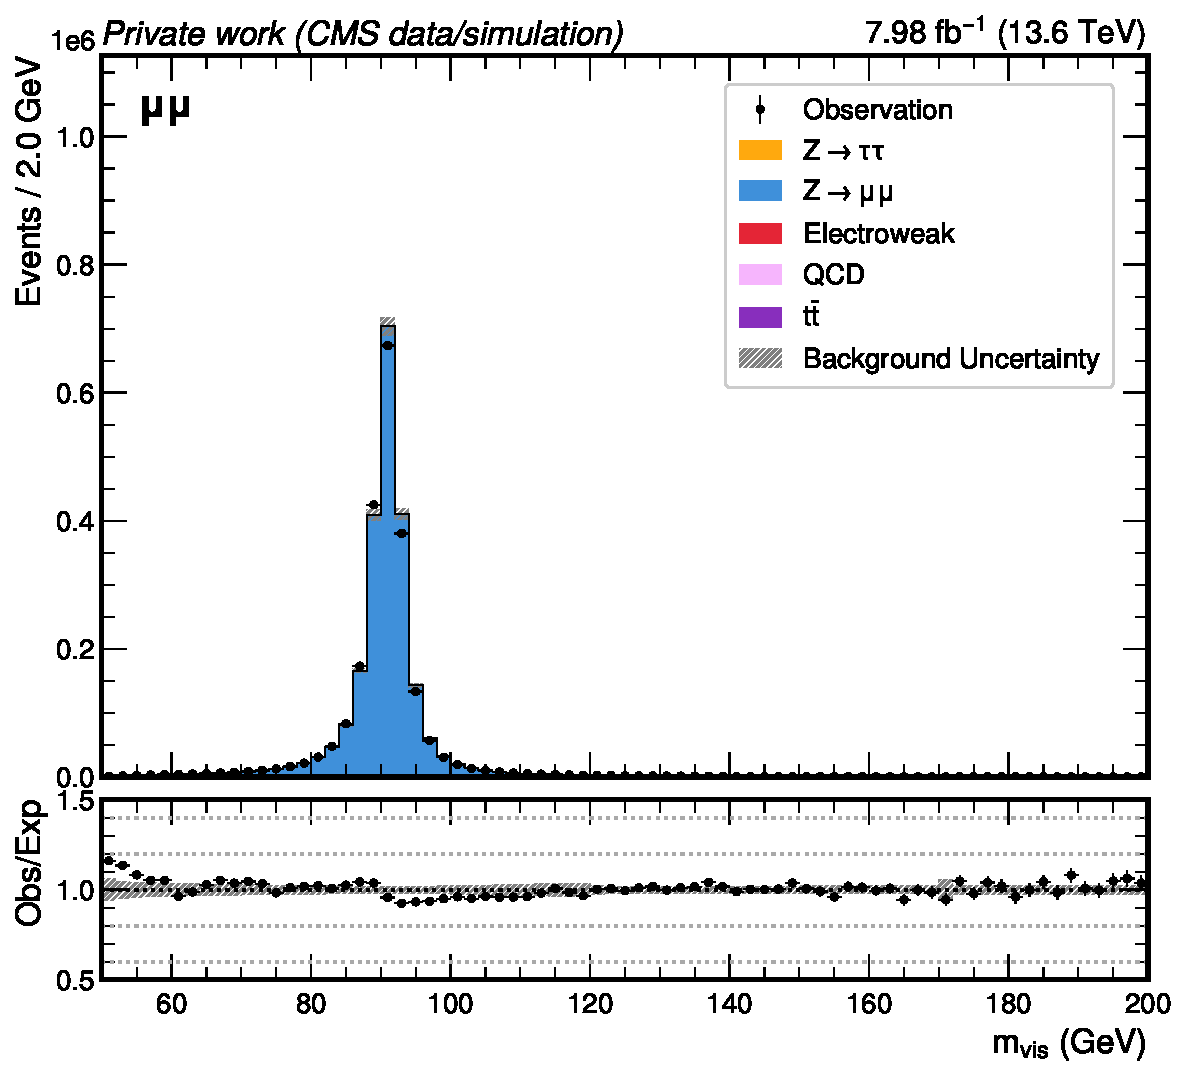
\includegraphics[width=\textwidth]{Figures/Chapter7/zpt_mvis_without.pdf}
            \caption{}
        \end{subfigure}
        \begin{subfigure}[b]{0.49\textwidth}
            \centering
            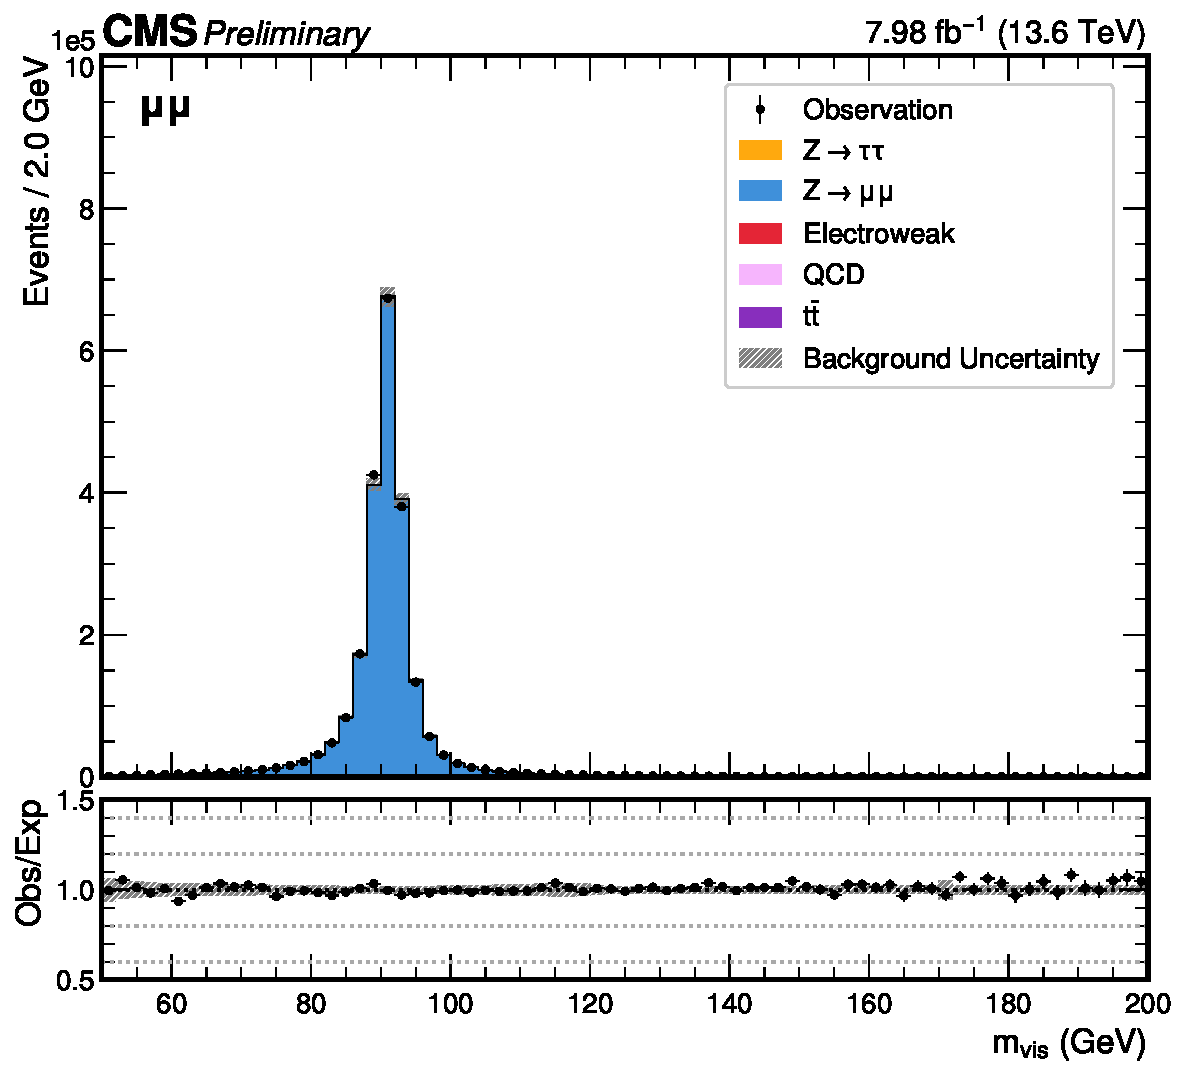
\includegraphics[width=\textwidth]{Figures/Chapter7/zpt_mvis_with.pdf}
            \caption{}
        \end{subfigure}

        \vspace{0.5cm}

        \begin{subfigure}[b]{0.49\textwidth}
            \centering
            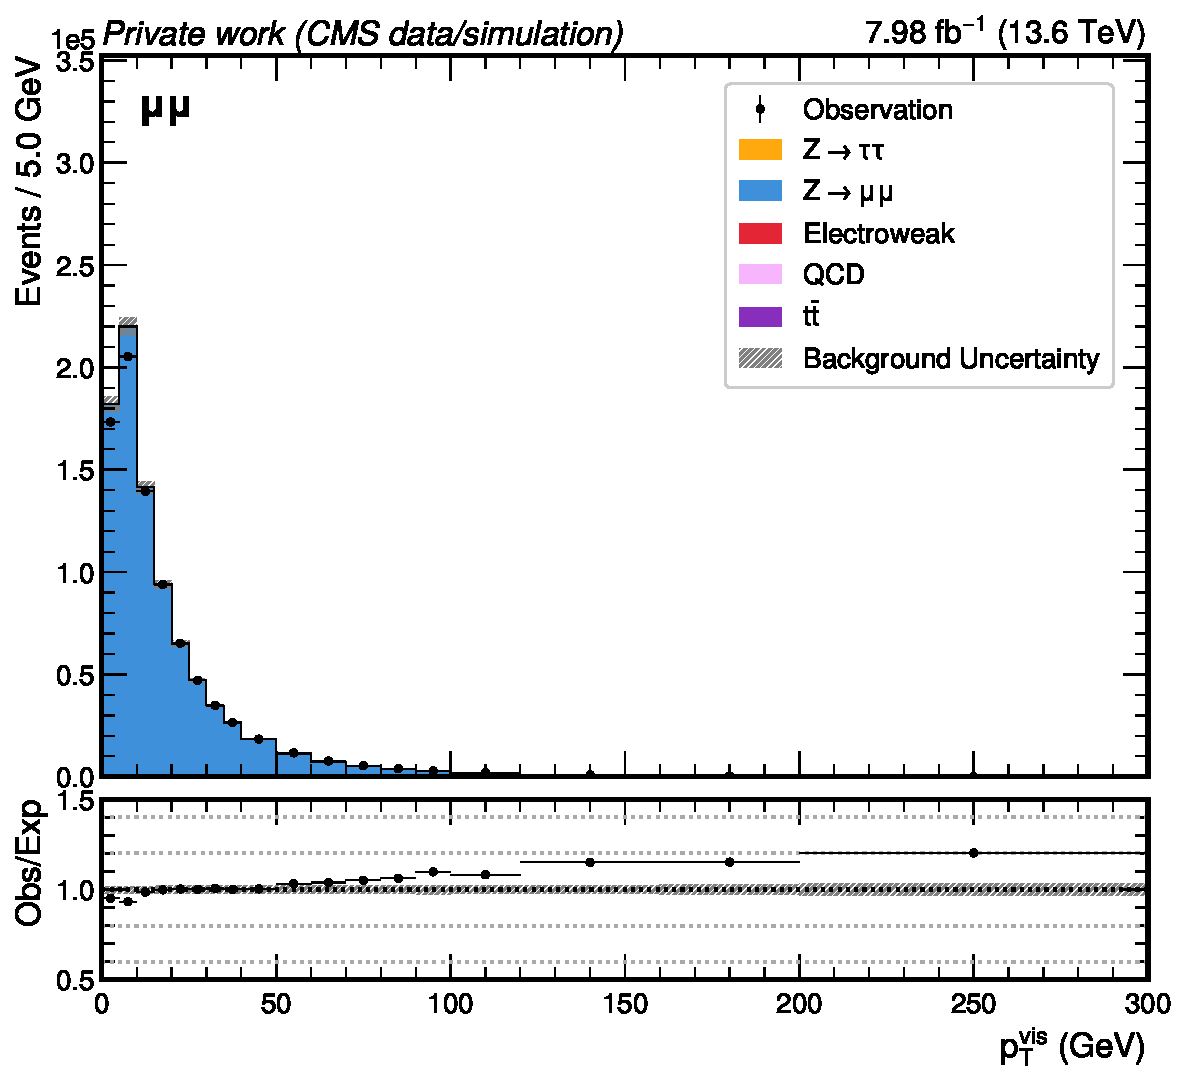
\includegraphics[width=\textwidth]{Figures/Chapter7/zpt_ptvis_without.pdf}
            \caption{}
        \end{subfigure}
        \begin{subfigure}[b]{0.49\textwidth}
            \centering
            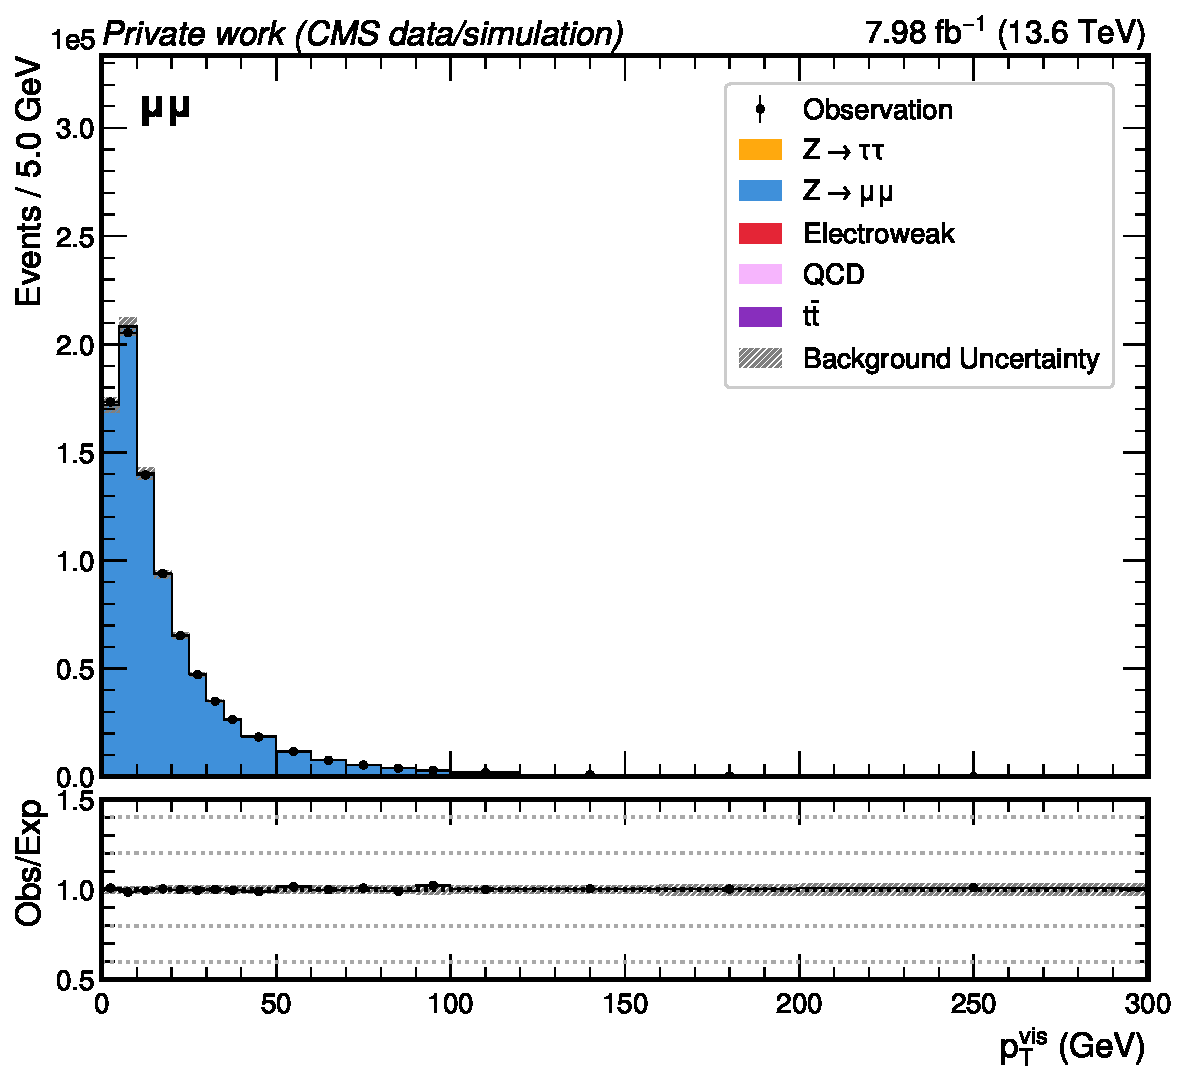
\includegraphics[width=\textwidth]{Figures/Chapter7/zpt_ptvis_with.pdf}
            \caption{}
        \end{subfigure}
    \caption[Reweighting validation in $Z/\gamma^* \to \mu\mu$ events.]{Validation of the $\PZ \, \, p_\text{T}$-mass reweighting in $Z/\gamma^* \to \mu\mu$ events. Shown are $m_\text{vis}$ distributions \textbf{(a)} before and \textbf{(b)} after reweighting, and $p_\text{T}^\text{vis}$ distributions \textbf{(c)} before and \textbf{(d)} after.}

    \label{Figure:Chapter6_ZPT_Reweighting}
\end{figure}

\begin{figure}[!htbp]
        \centering
        % First row
        \begin{subfigure}[b]{0.49\textwidth}
            \centering
            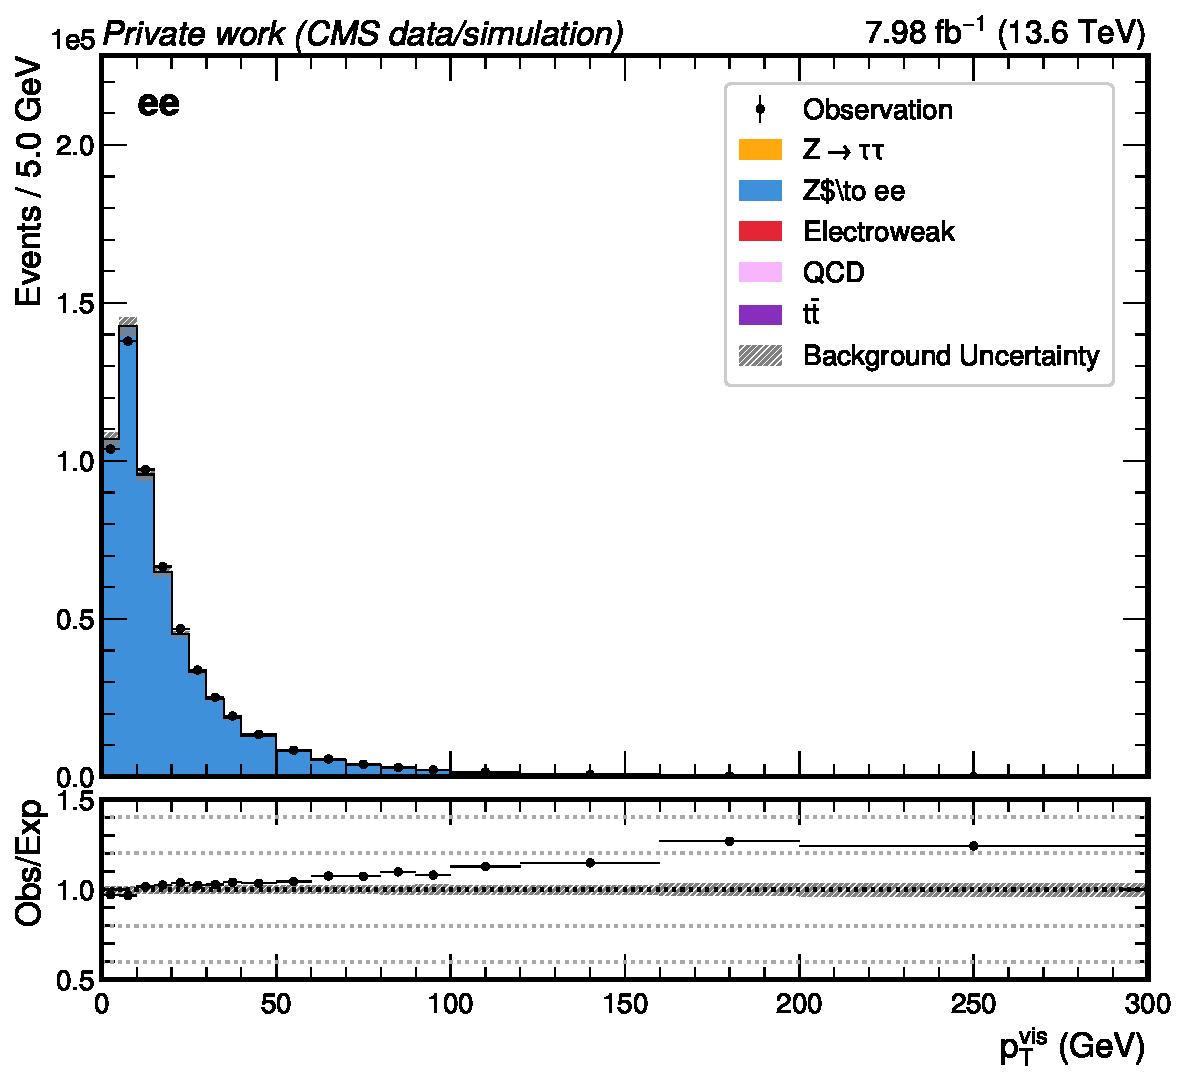
\includegraphics[width=\textwidth]{Figures/Chapter7/zpt_ee_ptvis_without.pdf}
            \caption{}
        \end{subfigure}
        \begin{subfigure}[b]{0.49\textwidth}
            \centering
            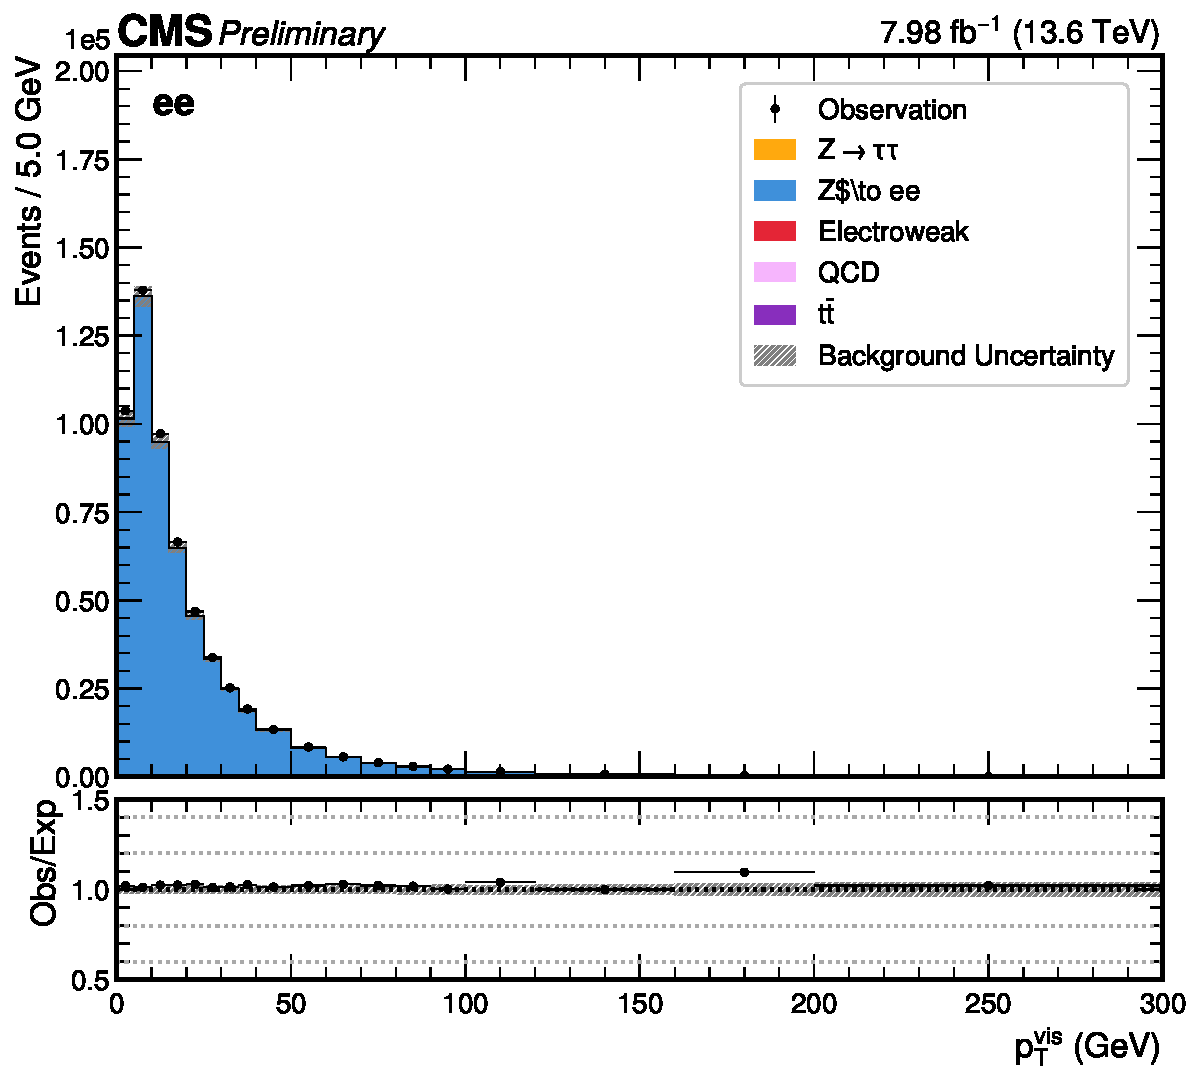
\includegraphics[width=\textwidth]{Figures/Chapter7/zpt_ee_ptvis_with.pdf}
            \caption{}
        \end{subfigure}
    \caption[Closure test of $\PZ \, \, p_\text{T}$-mass reweighting in $Z/\gamma^* \to ee$ events.]{Closure test of the $\PZ \, \, p_\text{T}$-mass reweighting in $Z/\gamma^* \to ee$ events. Distributions of $p_\text{T}^\text{vis}$ are shown \textbf{(a)} before and \textbf{(b)} after reweighting.}

    \label{Figure:Chapter6_ZPT_Reweighting_ee}
\end{figure}

\section{Background modelling}
\label{Section:Chapter7_Background_Modelling}


% Notes to Remember:
% 1. Variables not used to bias the BDT e.g. \deltaphi (differs between scenarios)